\chapter{Entwurf einer Bewertungsmatrix}
\label{ch:matrix}

Um die verschiedenen CAPTCHA-Arten effektiver bewerten zu können, soll eine Bewertungsmatrix entwickelt werden.
Hierzu wird zuerst der Stand der Wissenschaft hinsichtlich bereits vorhandener Bewertungsmatrizen betrachtet
und wie diese auf den vorliegenden Anwendungsfall anzuwenden sind.

Anschließend werden die Kategorien Bedienfreundlichkeit, also wie einfach die Tests auszufüllen sind, Accessibility, technische Umsetzbarkeit
und Sicherheit näher erläutert und es werden Fragen festgelegt, anhand derer man die Bewertung vornehmen kann.

Basierend auf diesen Kategorien können Punkte von 0 bis 10 vergeben werden.

\section{Stand der Wissenschaft}
\label{ch:matrix:sdw}

Es gibt bereits Methoden zur Bewertung von CAPTCHA.

In ihrem Paper ``A survey of research on CAPTCHA designing and breaking techniques'' beschreiben Zhang et al. das Design
und mögliche Angriffe verschiedener CAPTCHA-Technologien – textbasiert, bildbasiert und audio-/videobasiert.
Diese werden basierend auf Benutzerfreundlichkeit, Stabilität, ihren Stärken und Schwächen bewertet.  
Dabei wird festgelegt, dass CAPTCHAs als gut bezeichnet werden können, wenn diese von Menschen in über 90\% der Fälle gelöst werden können,
von Maschinen hingegen in weniger als 1\% der Fälle.
Quellen für diese Metrik sind Paper aus dem Jahre 2005 und 2008. \cite[p.75]{surveyofresearch}
Seitdem gab es weitreichende Entwicklungen im Bereich der künstlichen Intelligenz.

\dots
\dots

%Da es sich bei Veröffentlichung bereits um ein 10 Jahre altes Paper handelte, ist the accuracy of this statement fragwürdig 
%(schreib das mal in normal wenn du denken kannst).
%Die Metrik zur Bewertung der CAPTCHA wird unzureichend erklärt imo, ich hab aber auch nicht alles gelesen lul

\section{Bewertungsaspekte}
\label{ch:matrix:aspekte}
Die gegebenen Kategorien wurden gewählt, um einerseits Fokus auf die verschiedenen Aspekte der Nutzererfahrung legen zu können,
andererseits jedoch auch nicht die Sicherheit als initialen Grund für die Verwendung von CAPTCHAs außer Acht zu lassen.

Um die Bewertung zu erleichtern, werden je Kategorien einige beispielhafte Leitfragen angegeben, welche bei Bedarf auch angepasst werden können.
In diesem Fall sollte dies jedoch für alle zu betrachtenden Techniken getan werden, um die Vergleichbarkeit zu gewährleisten.

Durch die Vergabe von Punkten von 1 bis 10 je Kategorie ergibt sich so ein maximaler Score von 10.
Die Höhe der Punktzahl orientiert sich an eventuellen Abzügen, die durch Mängel in den jeweiligen Kategorien entstehen.

\subsection{Bedienfreundlichkeit}
\label{ch:matrix:aspekte:Bedienfreundlichkeit}
Bedienfreundlichkeit beschreibt, wie einfach es für Nutzer*innen ist, einen CAPTCHA auszufüllen.
Dies bedeutet, dass dies nicht zu lang dauern und auch nicht zu schwierig sein darf. 
Ist dies der Fall, werden bei der Bewertung abhängig vom Schweregrad Punkte abgezogen. %(diese seite mit der schlechten ux sehr gutes beispiel) 
Ein weiterer Aspekt, der zu Irritationen führen kann, sind zeitbegrenzte CAPTCHA. 
Diese laufen nach einer bestimmten Zeit ab und man muss die Seite neu laden und den Anmeldevorgang neu beginnen.
Auch hier ist ein Punktabzug nötig.

Die Betrachtung des Aufwands bei der Implementierung findet in Kapitel \ref{ch:matrix:aspekte:tu} statt, da dieser der technischen Umsetzbarkeit zuzuordnen ist.
Zu beantwortende Fragen können im diesem Kontext sein:
\begin{enumerate}
    \item Sind nur wenige Schritte nötig, um das CAPTCHA auszufüllen?
    \item Können Fragen oder Aufgaben eindeutig beantwortet beziehungsweise erfüllt werden? Gibt eine Fehlertoleranz?
    \item Gibt es keine zeitliche Begrenzungen?
\end{enumerate}
Können die Leitfragen nicht klar positiv beantwortet werden, führt das zu einer niedrigeren Bewertung des jeweiligen CAPTCHAs.
Eine hohe Bewertung bedeutet eine hohe Bedienfreundlichkeit. 

\subsection{Accessibility}
\label{ch:matrix:aspekte:accessibility}
Das Wörterbuch der Cambridge University definitiert Accessibility als ``$[$\dots$]$ the quality of being easy to understand $[$\dots$]$'' \cite{CACD:2008}

Dies stellt im Grunde auch die Definition für Accessibility im Kontext der zu entwickelnden Bewertungsmatrix dar:

\begin{enumerate}
\item Wie leicht lassen sich die verschiedenen CAPTCHA-Arten verstehen?
\item Sind sie für alle Personengruppen gleichermaßen nutzbar?
\item Welche Probleme könnten auftreten?
\end{enumerate}

Hierbei ist unter anderem zu beachten, dass CAPTCHA nicht nur an privaten PC-Arbeitsplätzen ausgefüllt werden,
sondern auf verschiedensten Geräten und mit unterschiedlichen Gegebenheiten.
Audiobasierte CAPTCHA können beispielsweise als störend wahrgenommen und deshalb nicht ausgefüllt werden,
wenn das Abspielen von Tönen andere stören könnte $($in öffentlichen Verkehrsmitteln, in Büros, \dots$)$,
oder das benutzte Gerät kann keinen Ton abspielen.
Nicht zu vergessen sind verschiedene körperliche Einschränkungen von Nutzer*innen,
die das Ausfüllen von CAPTCHAs erschweren oder gar unmöglich machen. Auch hier sind audiobasierte CAPTCHA zu erwähnen,
da diese für schwerhörige oder gehörlose Menschen nicht absolvierbar sind.
Ebenso müssen visuelle CAPTCHA für Screenreader optimiert werden, um sie für blinde Nutzer*innen nutzbar zu machen.
Auch andere visuelle Beeinträchtigungen, wie beispielsweise Rot-Grün-Schwächen, müssen beachtet werden.
Diese Aspekte führen jeweils zu Punktabzügen sofern sie auftreten.

Jedoch ist auch zu beachten, dass durch eine Kombination von einer visuellen 
und einer audiobasierten CAPTCHA-Methode auch blinde Menschen diese CAPTCHAs ausfüllen können. 
Dies wiederum wäre ein Pluspunkt. 
\begin{figure}
    \centering
    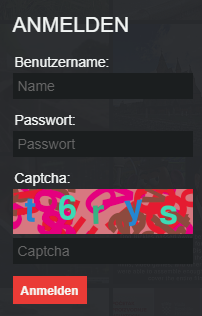
\includegraphics{gfx/mygraphics/pr0grammcaptcha.png}
    \caption{textbasiertes Captcha beim Login auf pr$0$gramm.com, das für Menschen mit Rot-Grün-Schwäche nur schwer zu erkennen ist}
\end{figure}

\subsection{Technische Umsetzbarkeit}
\label{ch:matrix:aspekte:tu}

Bei der technischen Umsetzbarkeit wird das Augenmerk auf die Implementation und Instandhaltung der Techniken gelegt.
Unzureichende Dokumentation kann die Implementation und eventuelles Debugging erheblich erschweren
und spielt deshalb eine wichtige Rolle bei der Auswahl.
Aus diesem Grunde werden je nach Qualität der Dokumentation gegebenenfalls Punkte abgezogen.
Gleiches geschieht, wenn der Ressourcenverbrauch sich stark erhöht, wenn die entsprechenden Methoden benutzt werden.
Auch bei der Implementierung kann es zu einer schlechteren Bewertung kommen, wenn diese sich kompliziert gestaltet und man viel an vorhandenem Code ändern muss,
um die jeweilige Technologie zu verwenden.

Es ergeben sich folgende Leitfragen:
\begin{enumerate}
    \item Ist die Dokumentation ausreichend? 
    \item Werden viele Ressourcen benötigt?
    \item Muss man vorhandenen Quellcode stark abändern?
\end{enumerate}
 
\subsection{Sicherheit}
\label{ch:matrix:aspekte:sicherheit}
Sicherheit ist der Hauptgrund für die Verwendung von Spam-Präventions\-techniken.
Wie bereits in den vorherigen Kapiteln erwähnt, werden CAPTCHAs und ihre Alternativen genutzt um bei dem Ausfüllen von Formularen Bots auszusortieren
und somit Spam zu vermeiden.
Es muss betrachtet werden, ob es schon Methoden zur Umgehung der CAPTCHAs gibt.
\begin{enumerate}
    \item Gibt es bereits bereits Algorithmen um den jeweiligen CAPTCHA zu lösen?
    \item Wie zugänglich ist die Umsetzung dieses Algorithmus? $($Kann jedermann ihn nutzen? Ist er ressourcenaufwändig?$)$
    \item Welche Erfolgsquote haben Angriffe?
\end{enumerate}

Die Punktevergabe richtet sich hierbei nach der Häufigkeit und Schwere von eventuellen Sicherheitslücken.
So werden beispielsweise mehr Punkte abgezogen, wenn es nicht nur einen Algorithmus gibt, welcher das entsprechende CAPTCHA löst,
sondern dieser zusätzlich noch leicht zu betreiben ist und eine hohe Erfolgsquote aufweist.

\section{Berechnung einer Metrik}
\label{ch:matrix:berechnung}
Bei der Berechnung einer Metrik auf Basis der entworfenen Matrix muss eine korrekte Gewichtung gewählt werden.
Diese ist nötig, um individuelle Entscheidungen für unterschiedliche Einsatzgebiete treffen zu können,
da die Bedürfnisse dieser stark unterscheiden können.

Die Gewichtung für jede Kategorie wird anteilig von 100 Prozent angegeben.
So wird es ermöglicht, präzise und individuell zu priorisieren.
Eine beispielhafte Bewertungsmatrix ist in \ref{beispielmatrix} gegeben.

\begin{table}[h!]
    \caption{Beispielhafte Bewertungsmatrix}
    \begin{center}
        \begin{tabular}{l|c|c|c}
            Kategorie                       & Bewertung & Gewichtung & \begin{tabular}{c}Gewichtete \\ Bewertung \end{tabular} \\\hline
            Bedienfreundlichkeit                         & 7         & 25\%       & 1.75       \\
            Accessibility                   & 10        & 10\%       & 1          \\
            Technische Umsetzbarkeit        & 3         & 30\%       & 0.9        \\
            Sicherheit                      & 9         & 35\%       & 3.15       \\ \hline
            \multicolumn{2}{l|}{Gesamtnote} & 100\%     & 6.8
        \end{tabular}
    \end{center}
    \label{beispielmatrix}
\end{table}





